\section{Les bases de données}
\label{sec:persistence}

\subsection{Concepts}
\label{subsec:persistence-concepts}

\begin{frame}
    \frametitle{Les concepts (1)}
    \begin{itemize}
        \item \textbf{Système de Gestion de Bases de Données} (SGBD / DBMS)\\
            Système logiciel qui permet de définir, créer, maintenir
            et contrôler des bases de données.
        \item \textbf{Base De Données} (BDD / DB)\\
            Collection organisée de données
            (plus ou moins structurées suivant le type de base de données).
        \item \textbf{Modèle de données} ou \textbf{Schéma}\\
            Description de l'organisation des données,
            il se trouve à l'intérieur de la base de données,
            et renseigne sur les caractéristiques de chaque type de donnée
            et les relations entre les différentes données.
    \end{itemize}
\end{frame}

\begin{frame}
    \frametitle{Les concepts (2)}
    \begin{itemize}
        \item \textbf{Entité} (table)\\
            Une entité est un \enquote{objet} étant décrit et pour lequel des données sont enregistrées.
        \item \textbf{Attribut} (champs ou colonnes)\\
            Un attribut est une caractéristique d'une entité susceptible
            d'être enregistrée dans la base de données.
            Dans le schéma les entités sont décrites comme un lot d'attributs.
        \item \textbf{Enregistrement} (ligne)\\
            Un enregistrement est une donnée composite qui comporte plusieurs
            champs dans chacun desquels est enregistrée une donnée.
    \end{itemize}
\end{frame}

\begin{frame}
    \frametitle{Les concepts (3)}
    \begin{itemize}
        \item \textbf{Association}\\
        Les associations désignent les liens qui existent entre différentes entités.
        \item \textbf{Cardinalité}\\
        La cardinalité d'une association entre deux entités A et B
        est le nombre de A pour lesquelles il existe un B et inversement.
        Celle-ci peut être un-à-un, un-à-plusieurs ou plusieurs-à-plusieurs.
    \end{itemize}
\end{frame}

\begin{frame}
    \frametitle{Modèle de données entité-association}

    Ce type de modèle est le plus couramment utilisé pour la conception de modèles de données.
    \begin{itemize}
        \item une base de données est un lot d'entités et d'associations ;
        \item une entité est un sujet concret, un objet, une idée ;
        \item un attribut est un renseignement concernant ce sujet ;
        \item à chaque attribut correspond un domaine (un ensemble de valeurs possibles) ;
        \item une association désigne un lien entre deux entités.
    \end{itemize}
\end{frame}

\begin{frame}
    \frametitle{Modèle de données entité-association}

    \centering
    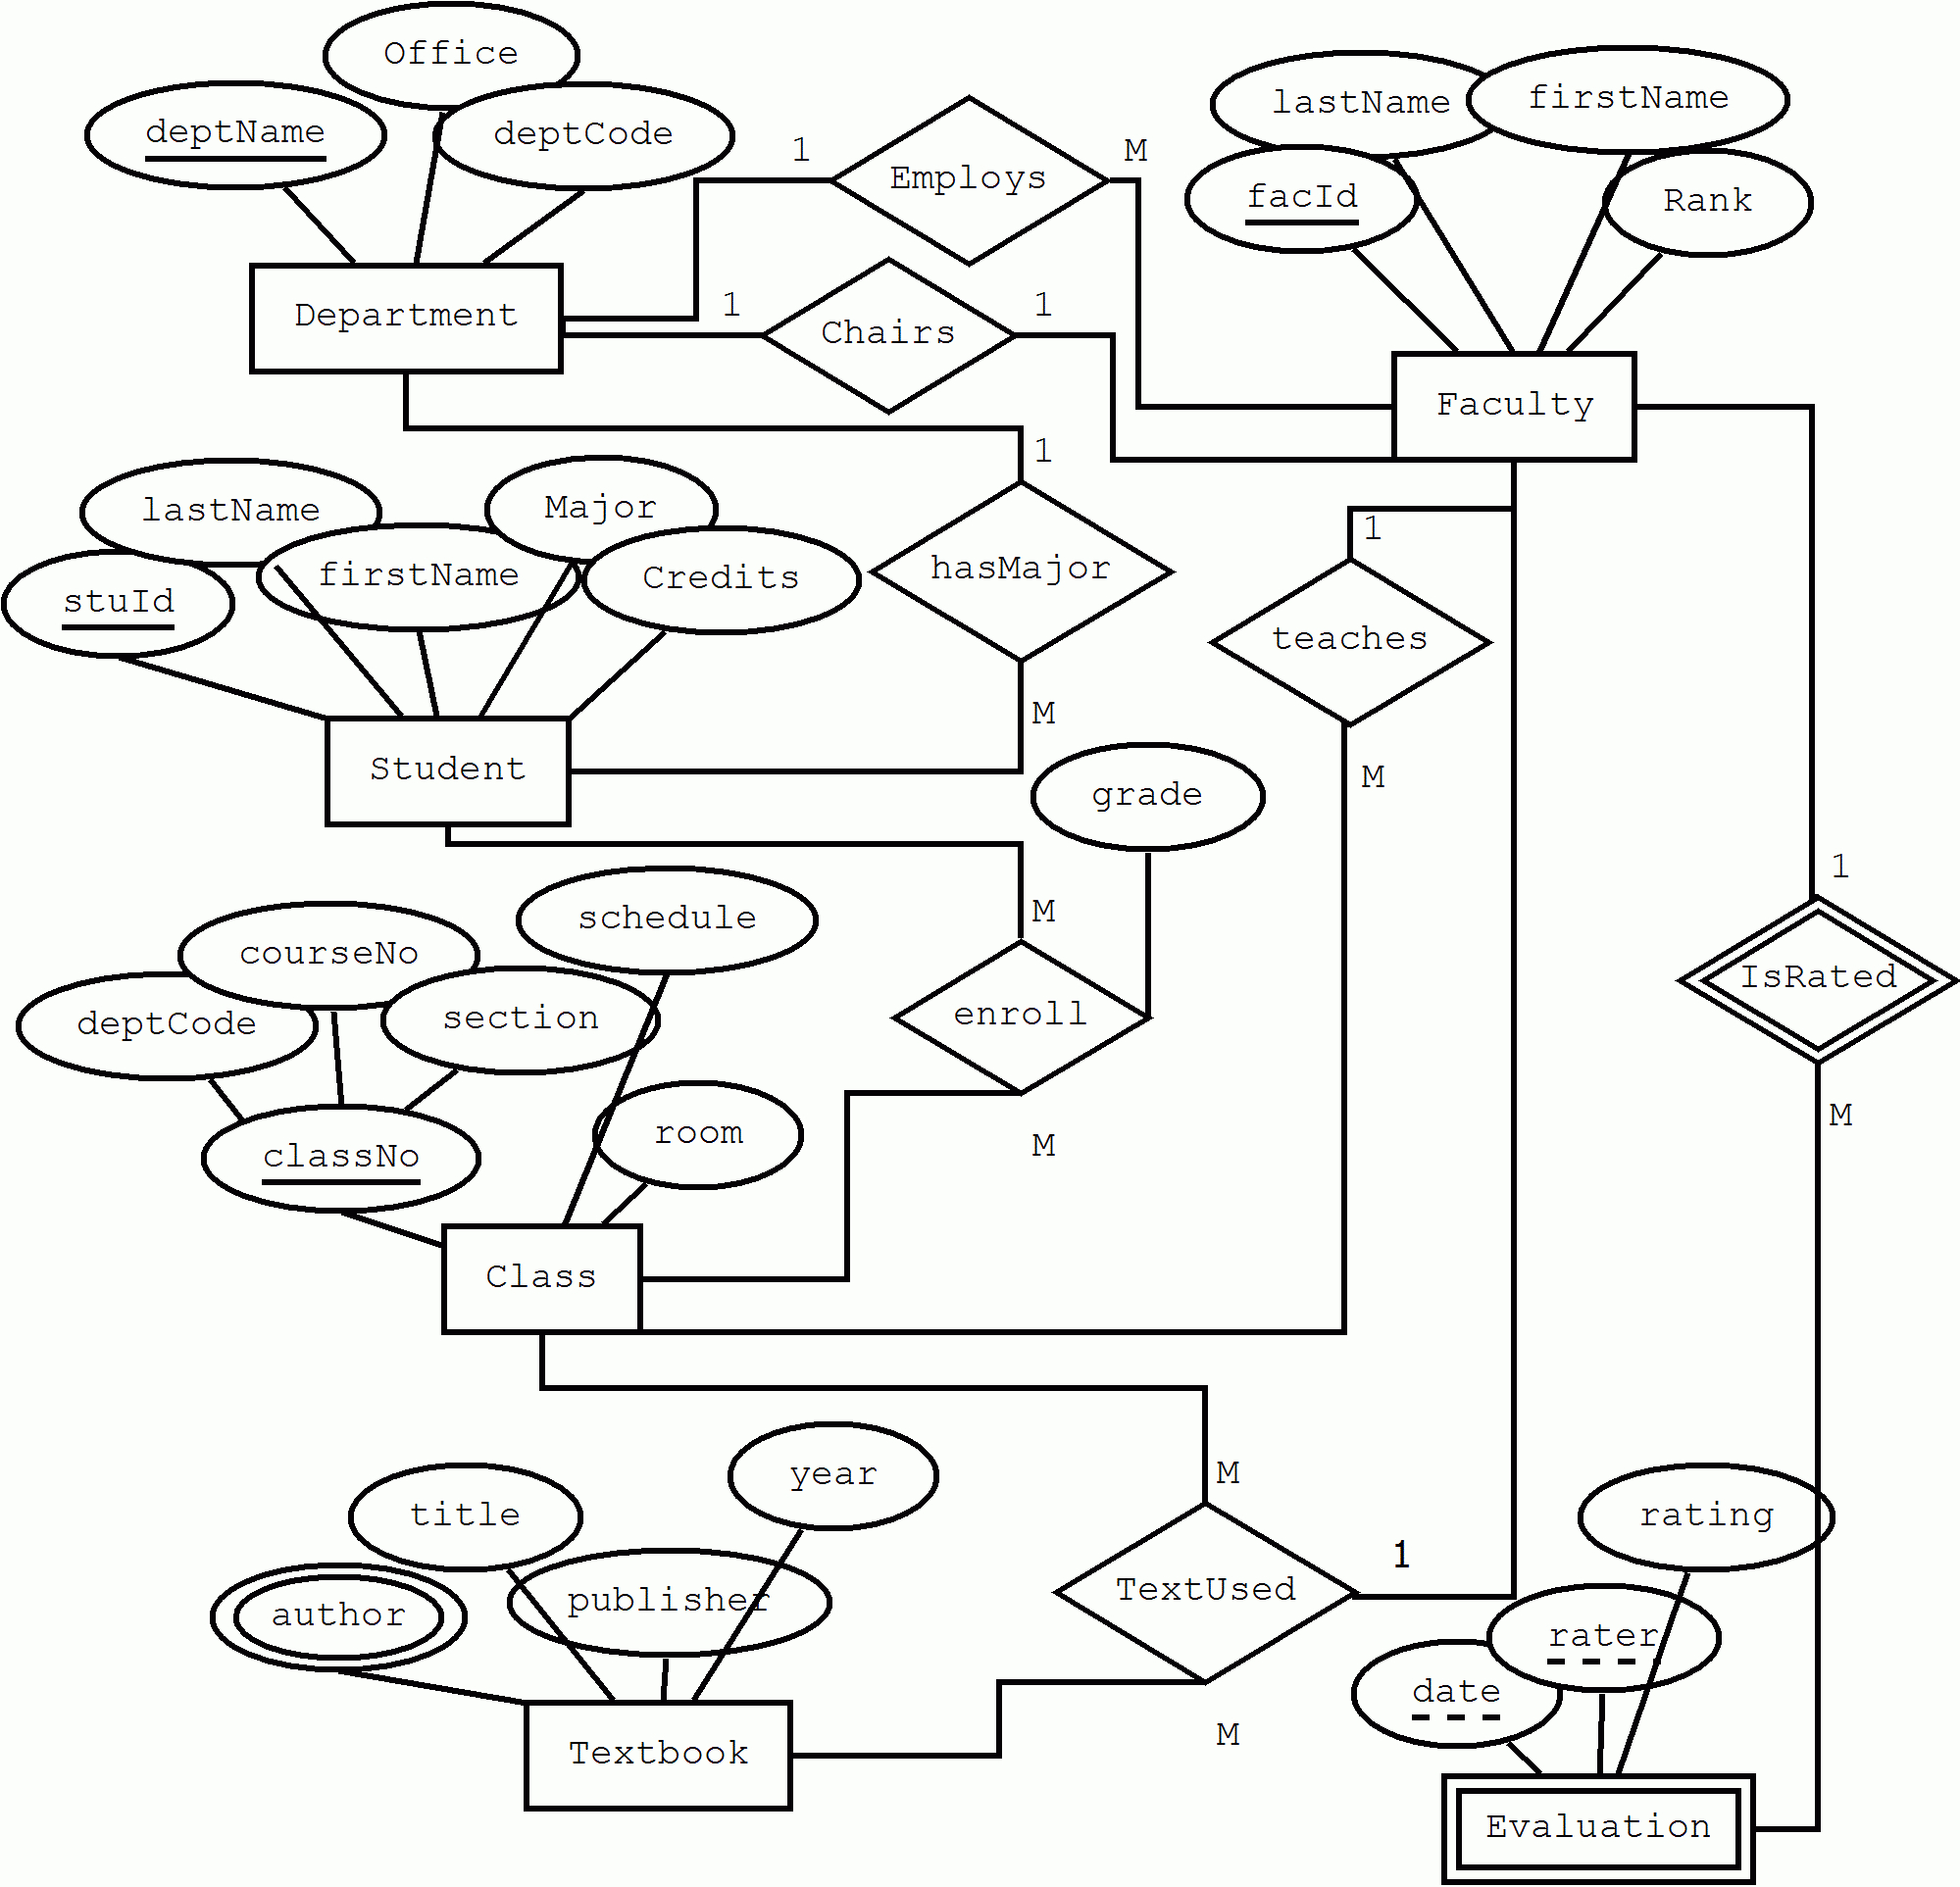
\includegraphics[width=0.5\linewidth]{figures/persistence/modèle-entité-association}
\end{frame}

\begin{frame}
    \frametitle{Modèle de données relationnel}

    C'est le type de modèle de données le plus couramment utilisé pour la réalisation d'une base de données.
    \begin{itemize}
        \item la base de données est composée d'un ensemble de tables (les relations) ;
        \item dans lesquelles sont placées les données ainsi que les liens.
        \item Chaque ligne d'une table est un enregistrement.
    \end{itemize}

    \bigskip
    Le modèle relationnel est basé sur deux instruments puissants :
    \begin{itemize}
        \item l’algèbre relationnelle (concept de relation en théorie des ensembles),
        \item la notion de produit cartésien.
    \end{itemize}

    \bigskip
    \emph{Une base de données relationnelle est organisée selon un modèle de données relationnel.}

\end{frame}

\begin{frame}
    \frametitle{Modèle de données relationnel}

    \centering
    \includegraphics[width=\linewidth]{figures/persistence/modèle-relationnel}
\end{frame}

\subsection{Requêtage}

\begin{frame}
    \frametitle{Langage de Requête Structuré (SQL)}

    Pour aller un peu plus loin :
    \begin{itemize}
        \item \texttt{DISTINCT} (\url{https://sql.sh/cours/distinct})
        \item \texttt{EXISTS} (\url{https://sql.sh/cours/where/exists})
        \item \texttt{HAVING} (\url{https://sql.sh/cours/having})
        \item \texttt{CASE} (\url{https://sql.sh/cours/case})
        \item \texttt{UNION} (\url{https://sql.sh/cours/union})
        \item \texttt{INTERSECT} (\url{https://sql.sh/cours/intersect})
        \item Sous-requête (\url{https://sql.sh/cours/sous-requete})
    \end{itemize}
\end{frame}

\begin{frame}
    \frametitle{Les index}

    En SQL, les index sont des ressources très utiles qui permettent d’accéder plus rapidement aux données.

    Avec un index placé sur une ou plusieurs colonnes le système d’une base de données peut
    rechercher les données d’abord sur l’index
    et s’il trouve ce qu’il cherche il saura plus rapidement
    où se trouve les enregistrements concernés.

    Ces petites ressources ont toutefois leurs inconvénients
    car cela occupe de l’espace supplémentaire dans la base de données.
    Par ailleurs, l’insertion de données est plus long
    car les index sont mis à jour à chaque fois que des données sont insérées.

    Généralement un index pourra être utilisé dans les requêtes utilisant
    les clauses WHERE, GROUP BY ou ORDER BY.
    Lorsqu’une base de données possède un grand nombre d’enregistrements
    (exemple: plusieurs milliers ou plusieurs millions de lignes)
    un index permet de gagner un temps précieux pour la lecture de données.

    % https://sql.sh/cours/index
\end{frame}

% Contrainte d'intégrité
% https://fr.wikipedia.org/wiki/Int%C3%A9grit%C3%A9_r%C3%A9f%C3%A9rentielle

\begin{frame}
    \frametitle{Plan d'exécution d'une requête}

    Dans le langage SQL,
    l’instruction EXPLAIN est à utiliser juste avant un SELECT
    t permet d’afficher le plan d’exécution d’une requête SQL.
    Cela permet de savoir de quelle manière le SGBD va exécuter la requête
    et s’il va utiliser des index et lesquels.

    \centering
    \smallskip
    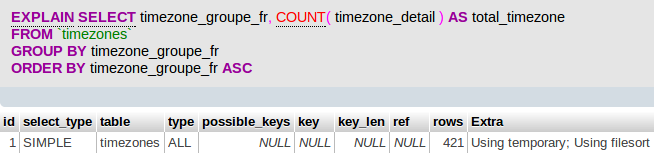
\includegraphics[width=0.7\linewidth]{figures/persistence/explain-1}

    \smallskip
    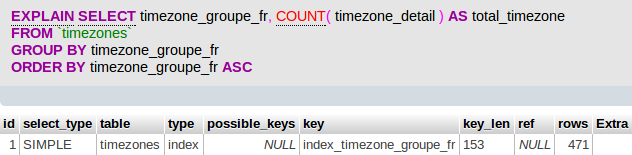
\includegraphics[width=0.7\linewidth]{figures/persistence/explain-2}
\end{frame}

\subsection{Types}

\begin{frame}
    \frametitle{Type de base de données}

    Bases de donnée relationnelles.

    \bigskip
    Les bases de données NoSQL (« pas seulement SQL ») sont des bases de données non tabulaires
    et stockent les données différemment des tables relationnelles.
    \begin{itemize}
        \item Les bases de données de documents stockent les données dans des documents similaires
        aux objets JSON.
        \item Les bases de données clé-valeur sont un type de base de données
        plus simple dans lequel chaque élément contient des clés et des valeurs.
        \item Les base de donnée orientée large colonnes larges stockent les données
        en se focalisant sur chaque attribut et en les distribuant.
        \item Les bases de données graphes stockent les données dans des nœuds et des arêtes.
    \end{itemize}

    % https://openclassrooms.com/fr/courses/4462426-maitrisez-les-bases-de-donnees-nosql/4462433-choisissez-votre-famille-nosql
\end{frame}

\begin{frame}
    \frametitle{MongoDB}
    \centering
    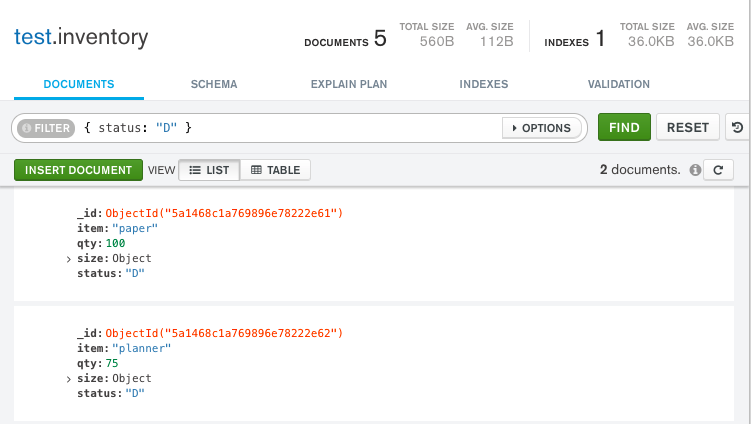
\includegraphics[width=0.7\linewidth]{figures/persistence/mongodb}
\end{frame}

\begin{frame}
    \frametitle{Neo4j}
    \centering
    \includesvg[width=0.45\linewidth]{figures/persistence/neo4j-graph}
\end{frame}

\begin{frame}
    \frametitle{Neo4j}
    \centering
    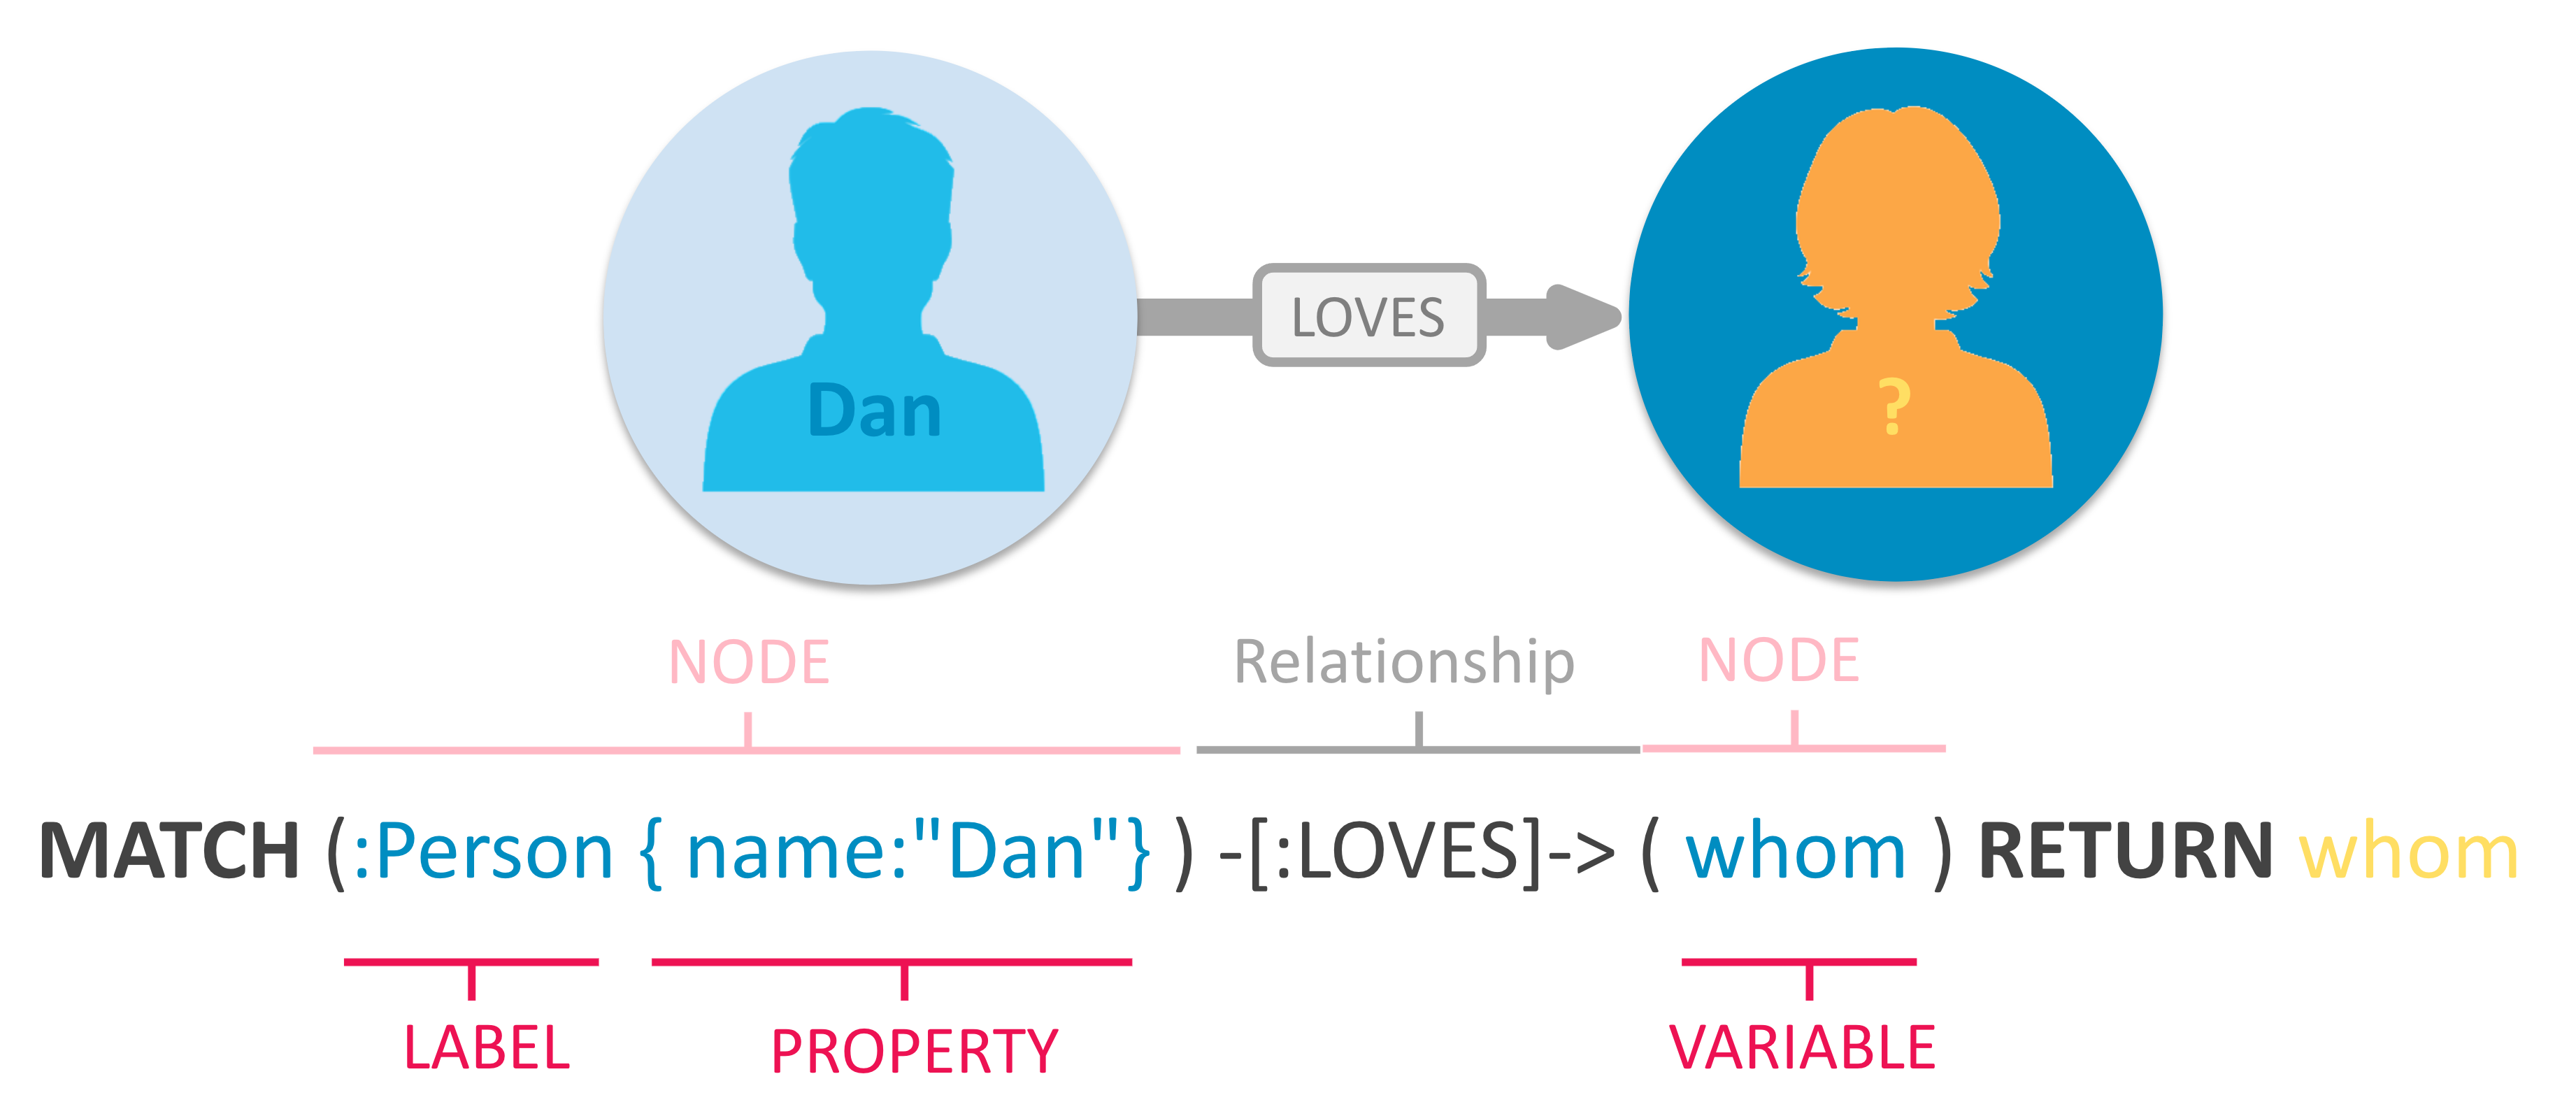
\includegraphics[width=0.7\linewidth]{figures/persistence/neo4j-cypher}
\end{frame}

%\begin{frame}
%    \frametitle{Elastic}
%\end{frame}
%
%\begin{frame}
%    \frametitle{OLAP}
%    % https://fr.wikipedia.org/wiki/Traitement_analytique_en_ligne#Relational_OLAP_(ROLAP)
%    % https://www.lebigdata.fr/olap-online-analytical-processing
%    % https://duckduckgo.com/?t=ffab&q=olap+relationnal&ia=web
%\end{frame}

\subsection{Propriétés}

\begin{frame}
    \frametitle{Transaction}

    En base de données,
    une transaction est un ensemble d’opération qui doit être effectué
    en respectant les propriétés d’atomicité, de cohérence, de durabilité et d’isolation (ACID).

    \bigskip
    Par exemple lorsqu’une transaction bancaire a lieu
    (un virement de 100 euros entre un compte A et un compte B),
    la transaction assure (et rassure) que le virement s’est bien déroulé correctement.
    Il n’y a pas eu d’erreur, tout a bien été enregistré,
    les 2 comptes ont bien pris note des mouvements et n’ont pas engendré d’erreur.
    Si un problème est détecté durant l’opération,
    la transaction est déconstruite et les données sont restaurées dans leur état initial.
\end{frame}

\begin{frame}
    \frametitle{Propriétés ACID}

    \begin{itemize}
        \item \textbf{Atomicité}\\
            garantit que chaque transaction est traitée comme une seule \enquote{unité},
            qui réussit complètement ou échoue complètement
        \item \textbf{Cohérence}\\
            garantit qu'une transaction ne peut faire passer la base de données que
            d'un état cohérent à un autre, en préservant les invariants de la base de données ;
        \item \textbf{Isolation}\\
            garantit que l'exécution simultanée des transactions laisse la base de données
            dans le même état que celui qui aurait été obtenu
            si les transactions avaient été exécutées séquentiellement.
        \item \textbf{Durabilité}\\
            garantit qu'une fois qu'une transaction a été validée,
            elle le restera même en cas de défaillance du système.
    \end{itemize}
\end{frame}

%\begin{frame}
%    \frametitle{Théorème CAP}
%    % https://en.wikipedia.org/wiki/Eventual_consistency
%    % https://fr.wikipedia.org/wiki/Th%C3%A9or%C3%A8me_CAP
%    % https://www.cl.cam.ac.uk/teaching//1213/Databases/db2013_L11_L12.pdf
%\end{frame}

\subsection{Accès aux données}

\begin{frame}
    \frametitle{Data Access Layer (DAL)}

    Une couche d'accès aux données (DAL) dans un logiciel est une couche d'un programme qui fournit
    un accès simplifié aux données stockées dans un stockage persistant.
\end{frame}

\begin{frame}
    \frametitle{Object–Relational Mapping (ORM)}

    Il s’agit d’une technique de programmation informatique qui permet de simplifier
    l’accès à une base de données en proposant à l’informaticien des « objets »
    plutôt que d’accéder directement à des données relationnelles.
    Ce niveau d’abstraction supplémentaire fait correspondre
    le monde objet et le monde relationnel.

    \bigskip
    Concrètement, l’ORM met à disposition des classes objet
    permettant de manipuler les bases de données relationnelles.
    Le développeur manipule ainsi des objets et
    l’ORM transforme le tout en requêtes compréhensibles par la base de données.
\end{frame}

\begin{frame}
    \frametitle{Object–relational impedance mismatch}

    Mathématiquement, l'approche objet est un graphe orienté.
    Une approche relationnelle est constituée de tuples dans des tableaux avec une algèbre relationnelle,
    formant un graphe non orientés.

    \begin{itemize}
        \item Incompatibilité entre les modèles objet et relationnel
        \item Différences de types de données
        \item Différences Structurelles et d'Intégrité
        \item Différences de Manipulation des Données
        \item Différences Transactionnelles
    \end{itemize}
\end{frame}

\begin{frame}
    \frametitle{Data Access Object}
    Le modèle d'objet d'accès aux données (DAO) est une abstraction de la persistance des données
    et est considéré comme plus proche du stockage sous-jacent,
    qui est souvent centré sur les tables.

    Fréquemment,
    les DAO correspondent aux tables de base de données,
    permettant ainsi un moyen plus simple d'envoyer/récupérer des données du stockage,
    masquant les requêtes SQL.
\end{frame}

\begin{frame}
    \frametitle{Repository}

    Un repository est un mécanisme d'encapsulation du comportement de stockage,
    de récupération et de recherche,
    qui émule une collection d'objets.

    En d’autres termes, un repository travaille à un niveau supérieur au DAO,
    plus proche de la logique métier d’une application.

    Un repository peut utiliser un DAO pour récupérer des données de la base de données
    et alimenter les objets métier.
\end{frame}

\begin{frame}
    \frametitle{Active Record}

    Un objet correspondant à une ligne dans une table encapsule
    l'accès à la base de données et ajoute une logique de domaine à ces données.

    Cette approche viole le principe de séparation des responsabilités.
\end{frame}